\section{An Application to Quantile Vector-Autoregressions}\label{sec:application}
For a real word data application, we apply the $\QVP$ prior to the quantile vector-autoregressive ($\QVAR$) model, as presented in \citet{chavleishvili2024forecasting}. The $\QVAR$ generalises the autoregressive quantile model of \citet{koenker2006quantile} to vector valued targets and is commonly used to examine the interactions of endogenous variables across their respective conditional distributions. $\QVAR$s represent an important policy tool for conducting stress-tests on financial systems, and more recently to quantify probability of tail events in macroeconomic time-series \citep{chavleishvili2023quantifying,chavleishvili2023measuring}. The literature has proposed many solutions to the multiple quantile function estimation problem (see \citet{hallin2017multiple} for an overview). Ambiguity arises because, unlike the univariate case, no single universally accepted mathematical framework for defining  a quantile function in multiple dimensions is accepted. The approach proposed in \citet{wei2008approach} is particularly convenient for economic models since the statistical identification assumption is also often defensible from the standpoint of economic theory \citep{chavleishvili2024forecasting}.
%

%
The $\QVAR$ of order one, written $\QVAR(1)$, takes the following form for $t=2,\dotsc,\mathcal{T}$: 
%
\begin{equation} \label{eq:QVAR-qform}
    Q_{\tau_q}(Y_t \mid \Psi_t) = \mathcal{B}_{\tau_q} + \mathcal{A}_{0,{\tau_q}} Y_t + \mathcal{A}_{1,{\tau_q}} Y_{t-1},
\end{equation}
%
where $Y_t = (y_{1,t},\dotsc,y_{m,t})^T \in \mathbbm{R}^{m}$, $\mathcal{B}_{\tau_q} = ({b}_{1}, \dotsc, {b}_m) \in \mathbbm{R}^m $ is a vector of intercepts, $\mathcal{A}_{1,\tau_{q}} \in \mathbbm{R}^{m \times m}$ is the coefficient matrix on the lag vector, and $\mathcal{A}_{0,\tau_q} \in \mathbbm{R}^{m \times m}$ is a contemporaneous impact matrix. Denote the entry of the $i$\textsuperscript{ith} row and $j$\textsuperscript{th} column of $\mathcal{A}_{1,\tau_q}$ by $a_{i,j,1,q}$. \citet{wei2008approach} show that under the assumption of a lower triangular structure to $\mathcal{A}_0$, one obtains valid multivariate quantile function estimates by estimating the system one equation at a time. With this, $\Psi_t$ is the information set at time $t$, and differs for each variable due to the lower triangular structure of $\mathcal{A}_{0,\tau_q}$: $\Psi_{1,t} = \left\{ Y_{t-1} , Y_{t-2} ,\dotsc  \right\}$, $\Psi_{i,t} = \left\{ Y_{i-1,t},\Psi_{i-1,t} \right\}$ for $i = 2,\dotsc,m$. 
%

Thus, following the steps in Sections~\ref{sec:likelihood}-\ref{sec:qvp-prior}, the probabilistic representation of the model for the $i$\textsuperscript{th} variable and $q$\textsuperscript{th} quantile of the $\QVAR(1)$ becomes:
\begin{IEEEeqnarray}{rl}\label{eq:centred_qvp}
     y_{i,t} & = b_{i,q} + \tilde{z}_{i,t}^{T}\tilde{a}_{i,q} + \mu_{i,q,t} + \epsilon_{i,q,t}^{y},\; \epsilon^{y}_{i,q,t}\sim\normal\left(0,\theta_q^2\sigma^{y}_{i,q}\omega_{i,q,t}\right) \label{eq:observation-equation-centred-qvar} \\
     \tilde{a}_{i,q} & = \tilde{a}_{i,q-1} + \epsilon^{\tilde{a}}_{i,q},\; \epsilon^{\tilde{a}}_{i,q} \sim \mvn\left(0,\Sigma_{i,q}\right),  \quad q  = 1,\dotsc,\mathcal{Q} \label{eq:state-equation-centred-qvar} \\
     \tilde{a}_{i,0} & \sim \mvn\left(0,\Sigma_{i,0}\right) \label{eq:starting-condition-cented-qvar},
\end{IEEEeqnarray}
where $\tilde{z}_{i,t}$ refers to the $i^{\mathrm{th}}$ information set $\Psi_{i,t}$ in vectorised form, $\vect{\Psi_{i,t}}$, and similarly $\tilde{a}_{i,q}$ vectorises the $i^{\mathrm{th}}$ row of coefficients. Note that this setup differs from the recent literature on multi-variate modelling of multiple quantiles using the multivariate $\mathcal{ALD}$ ($\mathcal{MALD}$). This is not further considered here since the $\mathcal{MALD}$ does not, without further modification, prohibit crossing of quantiles. And inference on the quantile covariance matrix is complicated due to its non-standard conditional posterior \citep{iacopini2023money}.

%
Representing quantile function~\ref{eq:QVAR-qform} in the sample space of $Y_t$ is convenient for the subsequent forecasting and causal analysis. Define $U_t = (U_{1,t},\dotsc,U_{m,t}) \in (0,1)^m$, such that each element is distributed independently as a uniform distribution. \citet{wei2008approach} show that if the joint distribution of $Y_t$ is absolutely continuous, there exists a one-to-one mapping between the sample space of $Y$ and the hyper-cube $\left(0,1 \right)^m$\footnote{This is known as the Rosenblatt transformation.}: 
\begin{equation} \label{eq:QVARasUnif}
    Y_t = \mathcal{B}(U_t) + \mathcal{A}_0(U_t) Y_t + \mathcal{A}_1(U_t) Y_{t-1},
\end{equation}
where, one can obtain the standard $\VAR$ like representation of the model by making the right hand side, a  function of a constant and lags only:
\begin{equation}
    Y_t = v(U_t) + \mathcal{C}(U_t)Y_{t-1},
\end{equation}
where $v(U_t) \equiv \left( \mathbbm{I}_m - \mathcal{A}_0(U_t) \right)^{-1}\mathcal{B}(U_t)$ and $\mathcal{C}(U_t) \equiv \left( \mathbbm{I}_m - \mathcal{A}_0(U_t) \right)^{-1}\mathcal{A}_1(U_t)$. Set in Equation~\ref{eq:QVARasUnif} $U_t = \tau_q$ for $t=2,\dotsc,\mathcal{T}$.\footnote{These inverses can be shown to always exists whenever the $\QVAR$ coefficients imply a stationary process, which is equivalent to the stationary conditions on parameter matrices of standard $\VAR$ models.} %The key insight is that with orderings that are frequently used in macroeconomics for $\mathcal{A}_0$, the conditional joint distribution can be estimated by quantile regression.
% 

The data set for this application, obtained from  \citet{chavleishvili2024forecasting} on Euro Area macrofinancial data, contains the industrial production growth-rate $(\IP)$, which measures real economic activity, and the composite indicator of systemic stress $(\CISS)$, representing a measure of financial health of the Euro Area.\footnote{For more examples of the $\CISS$ used in Growth-at-Risk models, see \citet{figueres2020vulnerable}, \citet{szendrei2023revisiting} or \citet{varga2025non} among others.} The time-series are plotted in Figure~\ref{fig:EmpAppData}. Data are monthly and available from January 1999 to July 2018. The goal of the study is to jointly forecast $\IP$ and $\CISS$ with the $\QVAR$ system and perform causal analysis of how the conditional distribution of $\IP$ responds to perturbations in the $\CISS$ indicator.
%
\citet{chavleishvili2024forecasting} give economic justification to a lower-triangular identification scheme where $\IP$ impacts $\CISS$ contemporaneously, but $\IP$ only impacts the $\CISS$ with a lag.\footnote{This identification assumption is implicit in \citet{adrian2019vulnerable} and many more studies that followed. Lower‐triangular identification entails that shocks are identified through how they propagate dynamically through the system of equations. This approach is widely used in macroeconomics because it yields a unique decomposition of structural shocks for location scale $\VAR$ models, often matching intuitive causal narratives \citep{sims1980macroeconomics}. } %Tibi: this is mentioned also in the QIRF section, so I commented this out. This is in line with the macro-financial linkage literature, which suggests that real economic activity reacts only in the tail of the conditional distribution to changes in financial conditions. 
%\dk{Let me know what you think about this. I would like to foreshadow this so that we don't need to spring this out at the reader in the QIRF section}.
%To decide on the ordering note that there is an identification assumption embedded in \citet{adrian2019vulnerable}, namely that financial conditions has no contemporaneous effects on GDP growth distribution. \citet{chavleishvili2024forecasting} use this assumption to order $\CISS$ after $\IP$ encoding that $\IP$ impacts $\CISS$ contemporaneously but $\CISS$ only impacts $\IP$ with a lag.

%Since previous studies find that real economic activity reacts only in the tail of the conditional distribution to changes in financial conditions \citep{adrian2019vulnerable}, \citet{chavleishvili2024forecasting} give economic justification to a lower-triangular identification scheme where $\CISS$ impacts $\IP$ contemporaneously, $\IP$ only impacts the $\CISS$ with a lag.
%Their findings reveal that financial shocks have a markedly asymmetric and persistent effect on the lower quantiles of industrial production. By incorporating both real and financial variables into its framework and utilizing established identification strategies from the VAR literature, the QVAR approach provides a robust and insightful tool for macroprudential analysis and stress testing in modern macroeconomics.

\begin{figure}
    \centering
    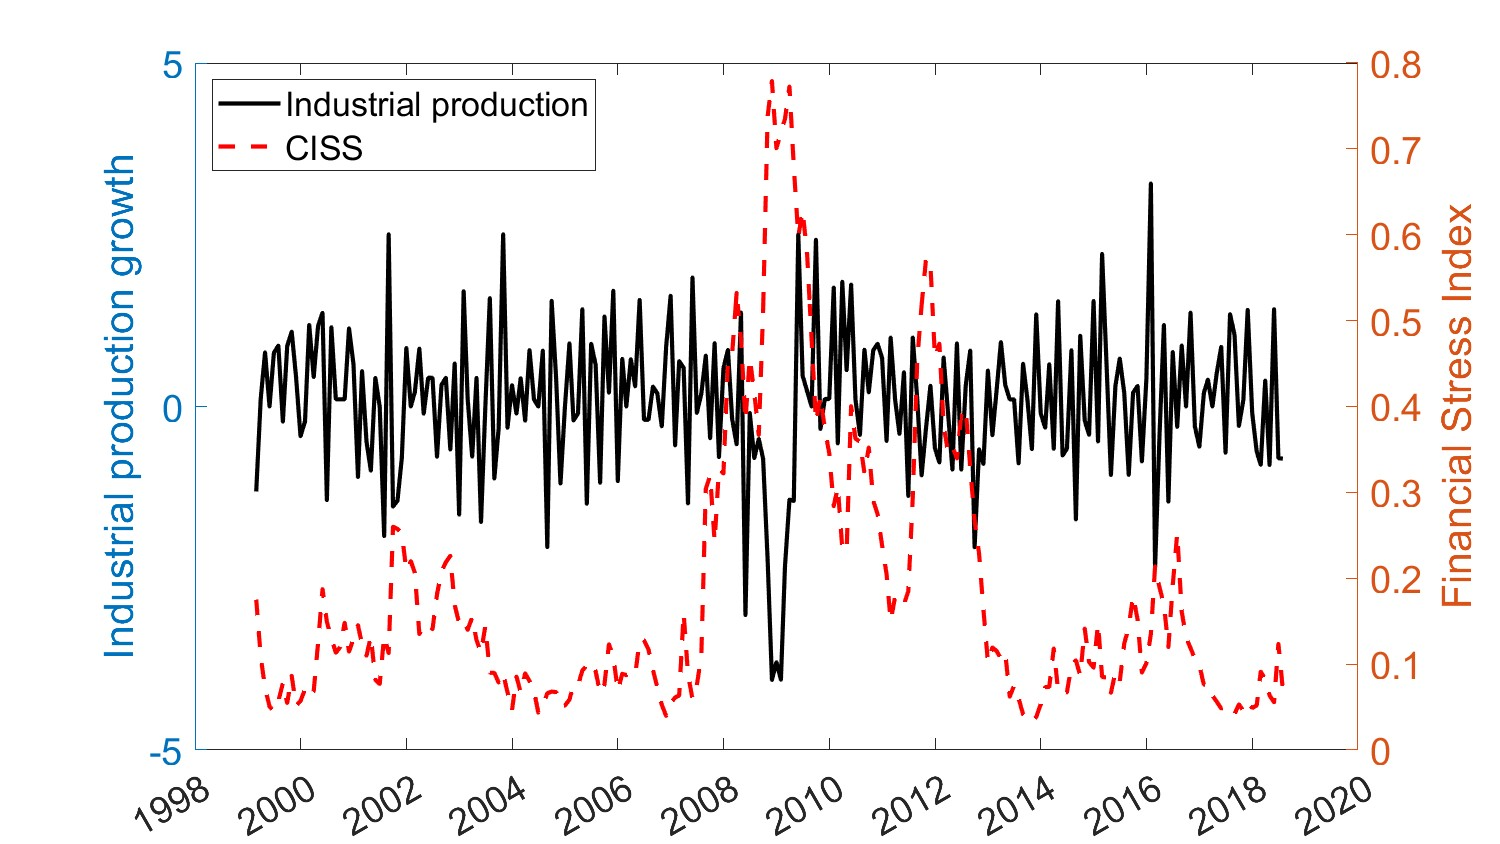
\includegraphics[width=0.9\linewidth]{Figures/FigureData.jpg}
    \caption{IP and CISS index for the available time-frame of January 1999 until July 2018}
    \label{fig:EmpAppData}
\end{figure}
%
We estimate the $\QVAR$ with the same set of priors as in Section~\ref{sec:simulation}. We generate h-step-ahead quantile predictions $Y_{t+h}$ for $h = 1,3,6$, which are evaluated with the $\QS$ score presented in Section~\ref{sec:simulation}. Then, we perform causal analysis common to the $\VAR$ applications in which we estimate the impulse response function of $\IP$ to a one-standard-deviation shock in the $\CISS$. %This true causal relationship can be retrieved from the parameter posteriors due to the lower-triangular identification assumption on $\mathcal{A}_{1}(U_t)$\footnote{\citet{chavleishvili2024forecasting} discuss the possibility of many other identification schemes, which we leave for future analysis}. This function is referred to as the impulse-response function.   
%

To retrieve quantile predictions, we follow the procedure given in \citet{chavleishvili2024forecasting}, however using the MCMC draws where appropriate. We summarise this in Algorithm~\ref{algorithm:forecasts}.
%As such we will estimate a QVAR model on the monthly euro area data from January 1999 to July 2018 of \citet{chavleishvili2024forecasting}. This dataset covers both stable and crisis periods, offering a comprehensive view of the euro area’s economic dynamics. The plots of these variables are shown in figure (\ref{fig:EmpAppData}). Here we will focus on the out-of-sample performance, QIRF, and the Stress test scenarios for the different priors. We will refrain from estimating the CQR for the QVAR application as it was only included in the Monte Carlo to glean the adaptability of the QVP prior.

% Algorithm 1
\begin{algorithm}[H] 
\caption{Algorithm for Multi-step Quantile Forecasts} \label{algorithm:forecasts}
\begin{algorithmic}[1]
\State \textbf{Input:} Data window: $\mathcal{T}_r$,  Data: $\left\{Y_t \right\}^{\mathcal{T}_{r }}_{t=1}$, posterior samples: $\left\{v(U)^{(s)}, \mathcal{C}(U)^{(s)}  \right\}_{s=1}^S$
\For{$n \in \left\{1,\dotsc,N\right\}$}
\For{$l \in {1,\dotsc,h}$}
    \State Randomly permute quantile level $U_{T_r+l}^{(n)}$ 
    \State Randomly draw from posterior sample $v(U_{T_r+l})^{(n)}, \mathcal{C}(U_{T_r+l})^{(n)}$
    \If{$l = 1$}
        \State Set $\hat{Y}_{T_r+1}^{(n)} = v(U_{T_r+1}^{(n)})^{(n)} + \mathcal{C}(U_{T_r+1}^{(n)})^{(n)} Y_{T_r}$
    \Else
        \State Set $Y_{T_r+l}^{(n)} = v(U_{T_r+l}^{(n)})^{(n)} + \mathcal{C}(U_{T_r+l}^{(n)})^{(n)} \hat{Y}_{T_r+l-1}^{(n)}$
    \EndIf
    \EndFor
\EndFor
\State \textbf{Output:} $ \boldsymbol{\hat{Y}} = \left\{\hat{Y}_{T_r+1}^{(n)},\dotsc, \hat{Y}_{T_r+h}^{(n)} \right\}_{n=1}^N$, where percentile $\tau_q$ of $\left\{ \hat{Y}^{(n)}_{T_r+l}\right\}_{n=1}^N$ yields the corresponding quantile prediction for period $t+l$.
\end{algorithmic}
\end{algorithm}
%
\subsection{Forecast Results}
Forecasts are produced on an expanding in-sample time-window $t = 1\dotsc,\mathcal{T}_r$, with initial in-sample period $\mathcal{T}_{\mathrm{start}}=96$ and $\mathcal{T}_{\mathrm{end}}=224$.
%
Quantile weighted $\QS$ scores for the $\QVAR$s are shown in Table~\ref{tab:ForcRes}. Similar to the results in Section~\ref{sec:simulation}, we show forecasting performance relative to the $\BQR$-$\QVAR$ model.%\footnote{\tibi{Footnote here stating SAVS forecasts use posterior means only.}\dk{can be made footnote to the table}}
%
\begin{table}[]
\centering
\resizebox{\textwidth}{!}{%
\begin{tabular}{ll|cccc|cccc|cccc}
 &  & \multicolumn{4}{c|}{h=1} & \multicolumn{4}{c|}{h=3} & \multicolumn{4}{c}{h=6} \\
 &  & CRPS & Centre & Left & Right & CRPS & Centre & Left & Right & CRPS & Centre & Left & Right \\ \hline
\multicolumn{2}{l|}{Equation 1: IP} &  &  &  &  &  &  &  &  &  &  &  &  \\
& $\BQR$  & 0.378 & 0.069 & 0.121 & 0.119 & 0.397 & 0.072 & 0.130 & 0.123 & 0.416 & 0.076 & 0.142 & 0.124 \\ \hdashline
& $\HSBQR$  & 91.1\% & 95.2\% & 88.3\% & 89.0\% & 90.7\% & 95.0\% & 88.3\% & 88.2\% & 90.1\% & 94.4\% & 88.7\% & 86.5\% \\
& $\BRW$  & 87.3\% & 92.9\% & 83.6\% & 84.5\% & 86.4\% & 92.3\% & 82.8\% & 83.2\% & 85.2\% & 91.5\% & 80.3\% & 83.2\% \\
& $\QVP$  & 86.3\% & 92.1\% & 83.1\% & 82.9\% & 86.4\% & 92.6\% & 83.2\% & 82.6\% & 85.0\% & 91.4\% & 80.3\% & 82.6\% \\
& $\NCQVP$  & 87.0\% & 92.8\% & 83.6\% & 83.7\% & 86.4\% & 92.3\% & 82.8\% & 83.2\% & 85.8\% & 92.0\% & 81.0\% & 83.5\% \\
& $\NCQVP_{\mathrm{SAVS}}$  & 87.4\% & 92.9\% & 84.5\% & 84.0\% & 86.6\% & 92.4\% & 83.0\% & 83.6\% & 84.8\% & 90.9\% & 79.3\% & 83.7\% \\
 \hline
\multicolumn{2}{l|}{Equation 2: CISS} &  &  &  &  &  &  &  &  &  &  &  &  \\
& $\BQR$  & 0.019 & 0.003 & 0.005 & 0.007 & 0.034 & 0.006 & 0.009 & 0.013 & 0.052 & 0.009 & 0.013 & 0.020 \\ \hdashline
& $\HSBQR$  & 91.9\% & 94.7\% & 89.9\% & 90.7\% & 95.4\% & 98.3\% & 92.3\% & 94.6\% & 96.8\% & 99.3\% & 92.6\% & 97.0\% \\
& $\BRW$  & 86.2\% & 90.9\% & 84.7\% & 82.7\% & 89.1\% & 94.1\% & 88.2\% & 84.9\% & 91.6\% & 96.6\% & 92.8\% & 86.3\% \\
& $\QVP$  & 85.7\% & 90.5\% & 84.2\% & 82.0\% & 88.5\% & 93.7\% & 87.9\% & 84.1\% & 90.9\% & 96.3\% & 92.1\% & 85.2\% \\
& $\NCQVP$  & 86.0\% & 90.6\% & 84.4\% & 82.4\% & 88.8\% & 93.9\% & 88.1\% & 84.3\% & 90.8\% & 96.1\% & 91.8\% & 85.2\% \\
& $\NCQVP_{\mathrm{SAVS}}$  & 91.2\% & 95.3\% & 89.9\% & 88.0\% & 91.9\% & 96.1\% & 90.1\% & 89.2\% & 91.5\% & 95.4\% & 93.3\% & 86.7\% \\
 \hline
\multicolumn{2}{l|}{Overall} &  &  &  &  &  &  &  &  &  &  &  &  \\
& $\BQR$  & 0.198 & 0.036 & 0.063 & 0.063 & 0.215 & 0.039 & 0.069 & 0.068 & 0.234 & 0.042 & 0.077 & 0.072 \\ \hdashline
& $\HSBQR$  & 91.1\% & 95.2\% & 88.4\% & 89.1\% & 91.1\% & 95.3\% & 88.6\% & 88.8\% & 90.8\% & 94.9\% & 89.0\% & 88.0\% \\
& $\BRW$  & 87.2\% & 92.8\% & 83.6\% & 84.4\% & 86.6\% & 92.4\% & 83.2\% & 83.3\% & 85.9\% & 92.0\% & 81.3\% & 83.7\% \\
& $\QVP$  & 86.3\% & 92.0\% & 83.2\% & 82.8\% & 86.6\% & 92.6\% & 83.5\% & 82.8\% & 85.7\% & 91.9\% & 81.2\% & 83.0\% \\
& $\NCQVP$  & 86.9\% & 92.7\% & 83.6\% & 83.6\% & 86.6\% & 92.4\% & 83.2\% & 83.3\% & 86.3\% & 92.5\% & 81.9\% & 83.8\% \\
& $\NCQVP_{\mathrm{SAVS}}$  & 87.6\% & 93.0\% & 84.7\% & 84.2\% & 87.0\% & 92.6\% & 83.4\% & 84.2\% & 85.6\% & 91.4\% & 80.4\% & 84.2\% \\
 \hline
\end{tabular}%
}
\caption{Forecast performance as measured by the weighted quantile score, $\mathrm{qwQS}$, see Equation~\ref{eq:qwQS}. Weighting schemes are $w_{q} = 1/\mathcal{Q}$ ($\QS$) which is equal to the $\mathrm{CRPS}$. $w_{q} = \tau_q(1-\tau_q)$ (Centre) places more weight the central quantiles, $w_{q} = (1-\tau_q)^2$ (Left) places more weight on left tail quantiles, $w_{\tau_q} = \tau^2_q$ (Right) places more weight on right tail quantiles. Performance is shown relative to $\BQR$ whose absolute performance shown above the dotted lines respectively. For the $\NCQVP_{\mathrm{SAVS}}$ only, the posterior means were used for this forecast exercise.}
\label{tab:ForcRes}
\end{table}
%
Several clear patterns emerge. First, joint‐quantile models consistently outperform independent quantile models ($\BQR$, $\HSBQR$), confirming the benefit of `partially pooling' information across quantiles observed in Section~$\ref{sec:simulation}$. Second, while $\HSBQR$ often excels at central quantiles, its tail performance is much worse than the $\QVP$ models, especially at longer forecast horizons. This is particularly visible for the $\IP$ variable. Third, the $\QVP$ prior variants can even outperform the $\BRW$ model, particularly in the tails. Here, integration over the parameter space with the Bayesian models induces more smoothness of the quantile function of the coefficients (see Section~\ref{app-sec:fig-posteriors}) and therefore reduces variance in the tails. Finally, forecast accuracy gets worse as the horizon increases which is a consequence of model parsimony and accumulation of forecast uncertainty. However, the loss in forecasts accuracy is less pronounced for joint estimation frameworks, particularly for the $\IP$ equation. % mitigate this loss more effectively than their independent counterparts, as seen by the joint estimators having comparatively more gains in performance as the forecast horizon increases especially for the IP equation.
%

In terms of crossing of the estimated (in-sample) quantiles, we find, similar to the Section~\ref{sec:simulation}, that the $\QVP$ priors almost completely eradicate the issue of crossing quantile curves (see Table~\ref{tab:cross-in-sample}). %\dk{Not sure the following statement is needed.}\tibi{I have the sentence here simply because I have read/heard arguments that if forecast is the interest you can always sort so who cares if quantiles cross in estimation. Our results clearly point that these priors lead to gains in forecasting as well. So there is no reason to not use them even if the goal is only forecasting. Can remove if you think it's not needed.} While shrinking towards non-crossing has benefits for inference, the forecast results (in conjunction with the in conjunction with the lower crossing incidence) highlights how methods that shrink towards non-crossing have forecast performance gains beyond sorting the $\BQR$ quantiles.\footnote{Note that out-of-sample forecasts will have a crossing incidence of 0 on account of taking the quantiles of the simulated multi-step paths.} 

%The IP equation (Eq. 1) presents a more challenging forecasting problem, with overall BQR $\QS$ scores higher than those for CISS. The $\BQR$ makes for a poor model, as all other models provide better forecast performance at all horizons and all parts of the distribution. The $\QVP$‐prior variants along with the $\BRW$ in particular yield uniformly better performance. This holds mostly also in comparison the the $\\HSBQR$, highlighting the value of joint-quantile estimation also for vecter-values quantile processes. The NCQVP variants stand out in tails-forecasting for $\IP$, where the extra regularisation allows for meaningful gains over even the $\BRW$ model.

%In the CISS equation (Eq. 2) the \HSBQR holds its own at the centre, achieving very low central‐quantile errors, but its tail performance remains comparatively inferior to the joint‐estimation methods. Both BRW and the QVP‐prior families continue to outperform independent quantile fits. Furthermore, the NCQVP variants deliver the largest relative improvements in the left and right tail weightings, highlighting their adaptability to asymmetric or heavy‐tailed patterns in the CISS.



%Given that the QVP prior variants produce as good (or better) out-of-sample fits as the BRW, we will refrain from reproducing results for the BRW. Furthermore, given that the \HSBQR yields worse performance than the joint quantile estiamtors, we will also not report results pertaining to the \HSBQR in the next sections.

\begin{table}[]
\centering
%\resizebox{1\textwidth}{!}{%
\begin{tabular}{r|ccc}
   & Eq. 1 & Eq. 2 & Overall \\ \hline
%$\BRW$ & 0.00\% & 0.00\% & 0.00\%  \\
$\BQR$ & 23.06\% & 50.26\% & 36.66\% \\
$\HSBQR$ & 16.83\% & 15.04\% & 15.94\% \\ \hdashline
$\QVP$ & 0.05\% & 0.14\% & 0.09\% \\
$\NCQVP$ & 0.20\% & 0.09\% & 0.15\% \\
$\NCQVP_{\mathrm{SAVS}}$ & 0.16\% & 0.05\% & 0.10\% \\ \hline
\end{tabular}%
%}
\caption{Crossing incidence (see Equation~\ref{eq:cross-i}) based on the entire sample. Estimates are based on the posterior mean of the coefficients.}
\label{tab:cross-in-sample}
\end{table}

\subsection{Quantile IRF}
%
$\QIRF$s measure the distributional causal effect of an unexpected change in $Y_{i,t}$ on $Y_{j,t}$ over some horizon $h = 1,\dotsc,W$. Such analyses are of interest to policy institutions like central banks, who tailor their policy instruments to the likelihood the potential paths real economic output take in relation to movements of the financial sector. Common to location-scale $\VAR$ analysis, the $\QVAR$ approach allows the analysis of such dynamic responses along particular points of the conditional distributions, in particular the tails.
%  
%This real-data application is based on a Euro-Area case study of \citet{chavleishvili2024forecasting} who investigate the dynamic quantile responses of industrial production ($\IP$) to worsening financial conditions, measured by the ($\CISS$) index. 
%

Denote by $Y_t^{*}$ a hypothetical `shocked' vector $Y_t$, to which $\iota \in \mathbbm{R}^m$ is added. As in \citet{chavleishvili2024forecasting}, we define $\iota$ as a vector of zeros, except entry $i$ which is equal to the shock's magnitude. The quantile impulse-response function at time point $t$ is defined as $\delta_{t}(U_t) \equiv Y_t^{*} - Y_t$.  \citet{chavleishvili2024forecasting} show that under the triangular identification scheme from above, this reduces to $\mathcal{D}(U_t)\iota$, where $\mathcal{D}(U_t) = \left( \mathbbm{I}_m - \mathcal{A}_0(U_t) \right)^{-1}$. The impulse response function for $h$-steps ahead is then given by: $\delta_{t+h}\left( U_{t+h} \vert U_t,\dotsc, U_{t+h-1}\right) = \prod_{g=1}^h\mathcal{C}(U_{t+g})\mathcal{D}(U_t)\iota$. We define the quantile response levels of interest of $\IP$ to be equal to $U_{\IP,t+g} = \tau = (0.05,0.1,\dotsc,0.95) \forall g$ while that of $\CISS$ are fixed to the median level, $U_{\CISS,t+g} = 0.5 \forall g$. Note, however, that for estimation of the coefficient-posteriors, it remains that both equations are estimated for all $\tau$.\footnote{We keep the quantile levels for the $\QIRF$ constant respective to each equation of the $\QVAR$. In principle, the quantile indices must stay constant across the horizons of the $\QIRF$.} The initial shock $\iota$ is set equal to a one standard deviation of the residuals at the median quantile of the $\CISS$ equation \citep{chavleishvili2024forecasting}. The previous literature finds that shocks to financial conditions have a more pronounced negative impact on the left tail of real economic output \citep{adrian2019vulnerable,chavleishvili2024forecasting}. It is therefore expected that the $\QIRF$s show a pronounced negative impact at low quantile levels that even out to 0 at high quantile levels.
%

Figure~\ref{fig:QIRF} shows the impulse response functions for the various quantile models for $h=1,\dotsc,30$. %In contrast to similar quantile functions for location-scale $\VAR$ models, here, we obtain a surface of impulse response functions.

% OLD
%Quantile Impulse Response Functions (QIRFs) extend the conventional impulse response framework by measuring the impact of structural shocks on different points of the forecast distribution rather than just on the mean. In essence, QIRFs capture how a shock affects various quantiles of an endogenous variable, revealing asymmetric and nonlinear dynamics that are especially important for stress testing and risk management. As such, while standard impulse response functions show the average effect of a shock, QIRFs allow researchers to trace the evolution of shocks through the entire distribution—highlighting, for instance, how extreme outcomes in the lower tail may be particularly sensitive to adverse financial shocks.

%In the QVAR framework of \citet{chavleishvili2024forecasting}, QIRFs are computed using a simulation-based recursive approach. First, the model is estimated via quantile regression, and structural shocks are identified through identification strategies used in the VAR literature. A shock is then introduced, typically by altering the distribution of one variable and the immediate effect is captured as the difference between the shocked and baseline forecasts as outlined in \citet{chavleishvili2024forecasting}. For subsequent periods, the effect of the shock is propagated through the system by multiplying it by the sequence of estimated state-transition matrices. This recursive procedure yields a series of QIRFs that illustrate how a one-time shock affects the entire forecast distribution over time.

\begin{figure}
    \centering
    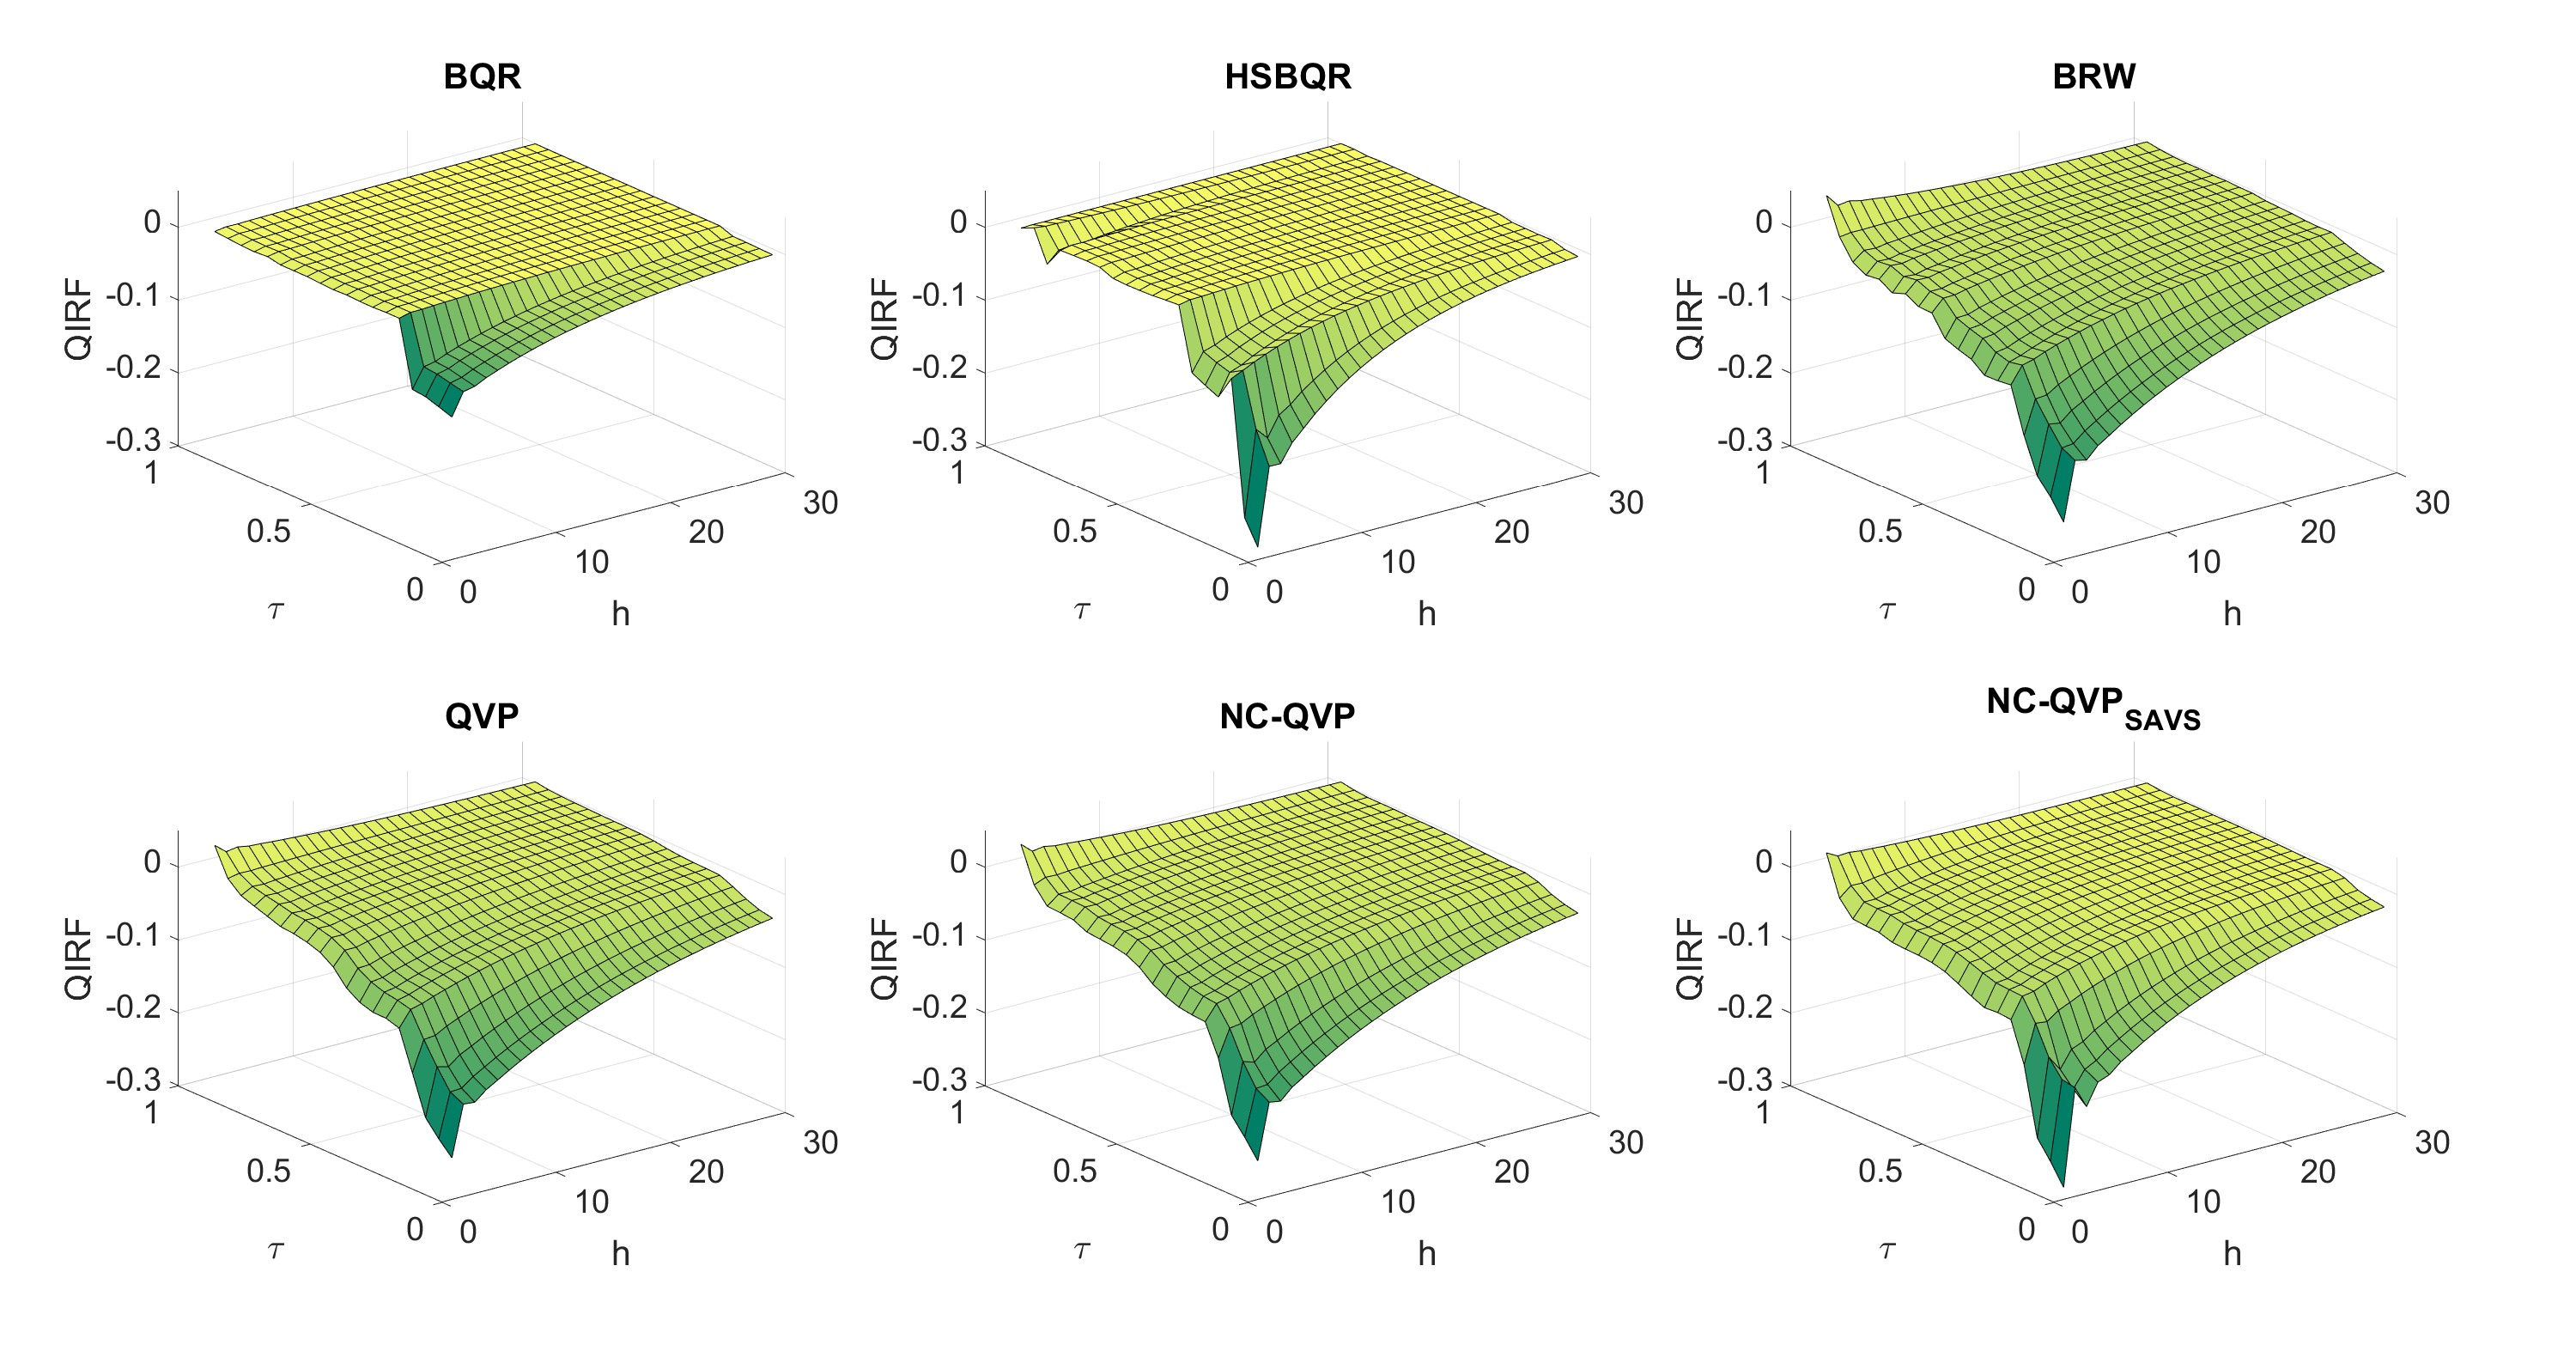
\includegraphics[width=\linewidth]{Figures/QIRF.jpg}
    \caption{$\QIRF$ surface of $\IP$ shown in response to one standard deviation shock to the $\CISS$ variable. Estimates are  based on the posterior means for quantile levels $\tau_q \in \left\{0.05,\dotsc,0.95\right\}$.}
    \label{fig:QIRF}
\end{figure}

\begin{figure}
    \centering
    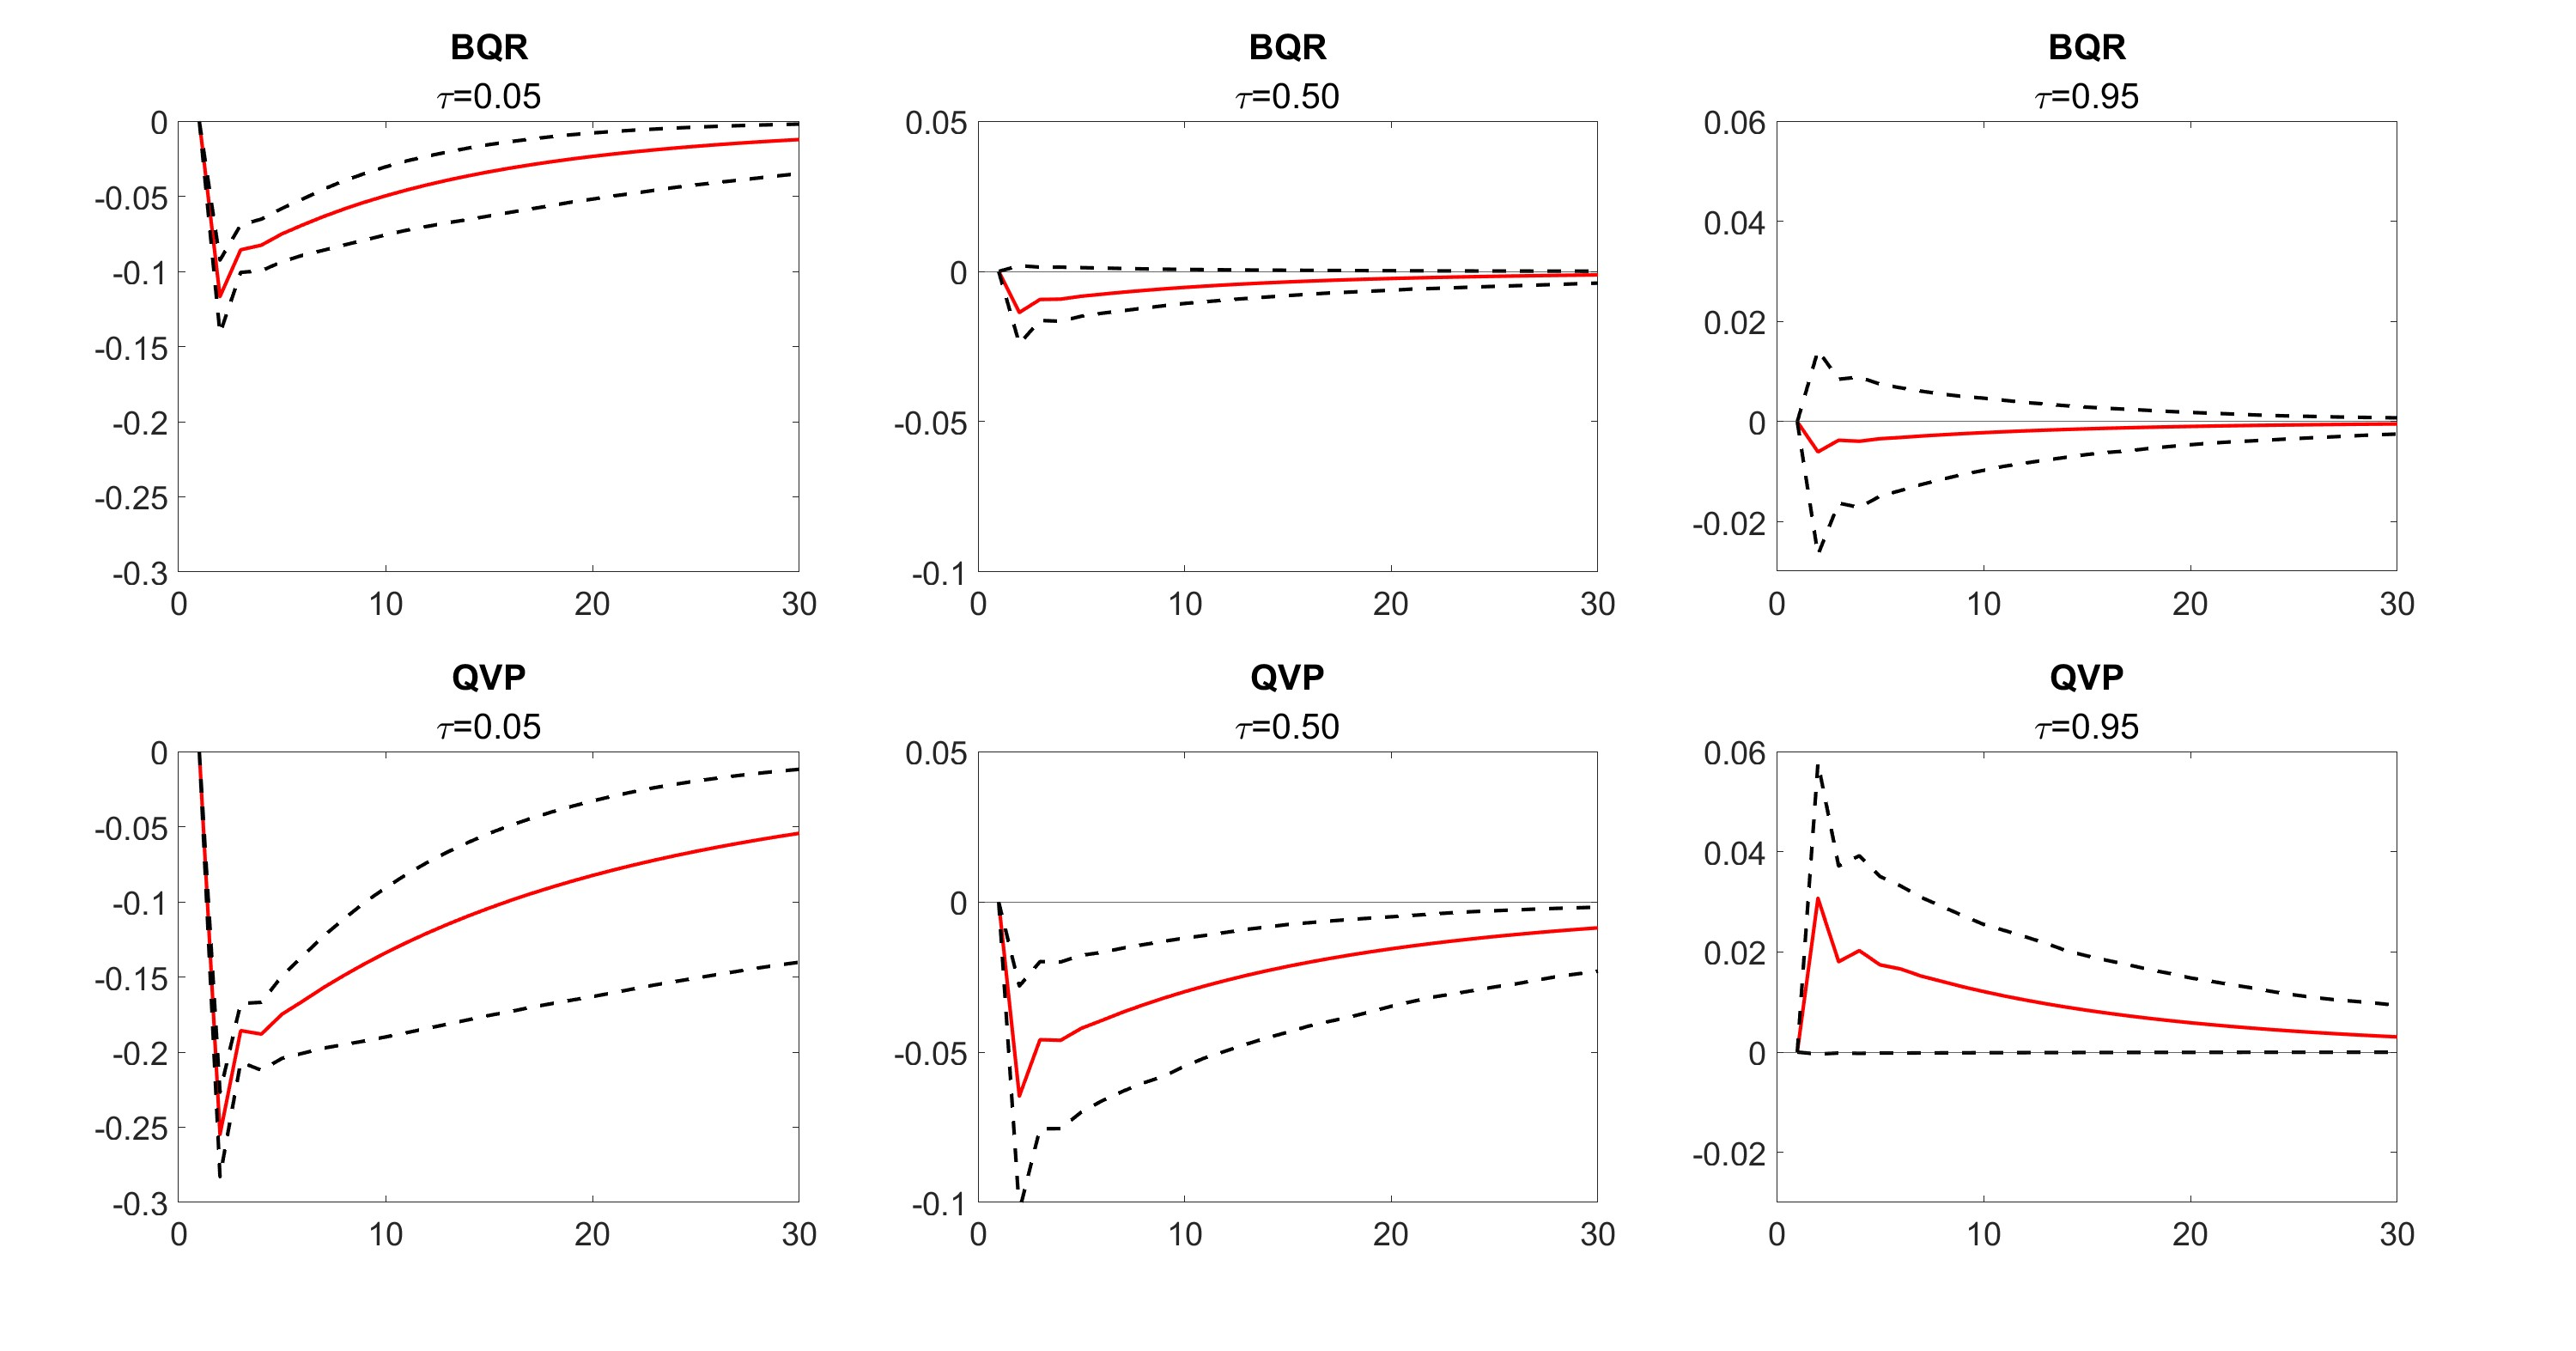
\includegraphics[width=\linewidth]{Figures/QIRF_QuantSpec.jpg}
    \caption{$\QIRF$ for $\BQR$ and $\QVP$ shown for selected quantiles $\tau_q \in \left\{0.05, 0.5, 0.95 \right\}$.}
    \label{fig:QIRFQuantSpec}
\end{figure}

%The different QVP prior QIRFs of IP to a one-standard deviation shock to the financial variable are shown in figure (\ref{fig:QIRF}), next to the QIRF of the BQR. The aim is to show how the entire distribution of industrial production growth responds over time when financial stress unexpectedly increases. In this way, one can trace how asymmetries in the transmission of financial shocks to the real economy evolve over time.

%
As expected, Figure~\ref{fig:QIRF} shows generally that all models estimate a pronounced negative impact of a shock to $\CISS$ to the left tail of $\IP$ with impulse response functions petering out to zero as the quantile level increases.
%
While the $\BQR$ and $\HSBQR$ models exhibit a notably sharp dip in the lower quantile only, the $\QVP$ models estimate a more gentle slope along the quantile levels. This is due to the $\QVP$ priors leading to smoother posterior quantile coefficient profiles - even compared to the $\BRW$ model.\footnote{Posteriors of the coefficients are shown in the appendix in figures \ref{fig:CoeffsIntercept}, \ref{fig:CoeffsContemp}, and \ref{fig:CoeffsLag}.}

%\dk{I don't directly see the connection between the following statement and the QVP models. Could you perhaps expand on this more if you think it's worth doing so?}\tibi{I think the only bit worth highlighting is what these qirfs mean for the distribution. I have been staring at graphs like this for years so for me it's obvious its a skewness effect with a location shift but someone not well versed might need this pointed out}\dk{Ok, I don't really understand the reasoning, and I think then people also wouldn't immediately make that connection. Let's talk about it} Furthermore, the $\QVP$ priors show larger negative dips at the lower tail compared to the BQR. Coupled with the additional smoothness of the QIRF along the quantile dimension, this leads to a situation where left tail skewness is increased and the location is shifted lower on account of a financial stress worsening, while for the BQR we only observe skewness increase.

Compared to \citet{chavleishvili2024forecasting}, we find that joint estimation of quantiles leads to significant differences in the $\QIRF$s, particularly at the median. Figure~\ref{fig:QIRFQuantSpec} shows the $\QIRF$ at selected quantiles for better visibility (including posterior uncertainty intervals). While the $\BQR$ model, in line with \citet{chavleishvili2024forecasting}, predicts no significant impact of the $\CISS$ shock at the median, the $\QVP$ model predicts a persistent negative one. Taken together, we confirm the previous literature's finding that post shock distributions of $\IP$ exhibit negative skewness, however, we also observe a significant downward location shift identified by the $\QVP$ models.  This highlights how using joint estimation, along with a prior that regulates information `pooling', can have a significant influence on the inference drawn from these models.

%Finally, there is a difference between the different priors in how long these effects in the QIRF persist. In particular we can see that the impact of financial stress remains even at h=30 for almost all the prior choices. These differences highlight how the choice of prior directly influences both the magnitude of the downturn in the lower quantile and the persistence of the shock's effect over time.
